\documentclass[9pt]{beamer}

\beamertemplatenavigationsymbolsempty
\renewcommand\mathfamilydefault{cmr}

\usepackage{pajmath}
\usepackage{booktabs}
\usepackage{colortbl}

\usepackage{tikz}
\usetikzlibrary{positioning,shapes.misc,calc,backgrounds,scopes} 
\usetikzlibrary{datavisualization}
\usetikzlibrary{datavisualization.formats.functions}
\tikzset{boxed/.style={
  thick,
  draw=black,
  top color=white,
  text height=1.5ex,
  text depth=.25ex
}}


\newcommand\lo{$-1$}
\newcommand\hi{$\phan1$}
\newcommand\ze{$\phan0$}
\newcommand\Ze{$\phan\Vzero$}

\title{Response Surface Methodology:\\Alternative Designs}
\author{BIOE 498/598 PJ}
\date{Spring 2021}

\begin{document}
\frame{\titlepage}

\begin{frame}{Why alternatives to the CCD?}

\begin{itemize}
	\item The CCD is excellent (and in many ways optimal) for RSM.
	\item Many alternatives have been developed to address one of two CCD shortcomings:
	\begin{enumerate}
		\item The CCD requires 5 levels for each factor.
		\item The CCD requires a lot of runs.
	\end{enumerate}
\end{itemize}
	
\end{frame}

\begin{frame}{Box-Behnken Designs (BBD)}

\begin{columns}
\begin{column}{0.7\textwidth}
	\begin{itemize}
		\item 3-level design with performance close to a CCD.
		\item Similar number of runs to a CCD.
		\item Built from $2^2$ factorials for each pair of factors.
		\item<3-> Nearly rotatable (rotatable for $k=$ 4 or 7).
		\item<3-> 3--5 center runs are recommended. (At least one center run is required for $k=$ 4 or 7).
	\end{itemize}
\end{column}
\begin{column}{0.3\textwidth}
	\onslide<2->{
		\begin{tabular}{ccc}
			\toprule
			$x_1$ & $x_2$ & $x_3$ \\
			\midrule
			\lo & \lo & \ze \\
			\lo & \hi & \ze \\
			\hi & \lo & \ze \\
			\hi & \hi & \ze \\
			\\
			\lo & \ze & \lo \\
			\lo & \ze & \hi \\
			\hi & \ze & \lo \\
			\hi & \ze & \hi \\
			\\
			\ze & \lo & \lo \\
			\ze & \lo & \hi \\
			\ze & \hi & \lo \\
			\ze & \hi & \hi \\
			\\		
			\Ze & \Ze & \Ze \\
			\bottomrule
		\end{tabular}
	}
\end{column}
	
\end{columns}

\medskip
{\footnotesize Note that in the bottom row \Vzero\ is a vector, i.e.\ a set of repeated center points.}
\end{frame}

\begin{frame}{The BBD is a spherical design}

\begin{columns}
\begin{column}{0.7\textwidth}
	\begin{itemize}
		\item All points in a BBD are on the edges, not the corners, of the design space.
		\item For $k=3$, all points are $\sqrt{2}$ away from the design center.
		\item<2-> The BBD is not good at predicting responses near the corners (\emph{extremes}) of the design space.
		\item<2-> Since the BBD is spherical and rotatable, ``ample'' center points should be used (Myers~2009).
	\end{itemize}
\end{column}
\begin{column}{0.3\textwidth}
	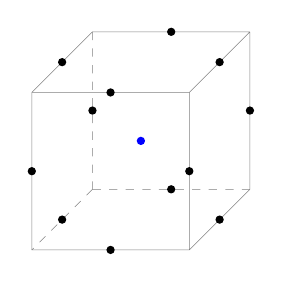
\begin{tikzpicture}
	\def\u{2}
	\def\cw{3pt}
	\begin{scope}[shift={(3,0)},scale=0.5]
		\draw [help lines] 
			(\u,\u,-\u) -- (-\u,\u,-\u) (\u,-\u,-\u) -- (\u,\u,-\u)
			(\u,\u,\u) -- (-\u,\u,\u) -- (-\u,-\u,\u) -- (\u,-\u,\u) -- (\u,\u,\u)
			(\u,\u,-\u) -- (\u,\u,\u)
			(-\u,\u,-\u) -- (-\u,\u,\u)
			(\u,-\u,-\u) -- (\u,-\u,\u);
		\draw [help lines,dashed]
			(-\u,-\u,-\u) -- (\u,-\u,-\u)
			(-\u,\u,-\u) -- (-\u,-\u,-\u)
			(-\u,-\u,-\u) -- (-\u,-\u,\u);
		\fill (\u,\u,0) circle (\cw) 
			  (-\u,\u,0) circle (\cw) 
			  (-\u,-\u,0) circle (\cw) 
			  (\u,-\u,0) circle (\cw)

			  (0,\u,\u) circle (\cw) 
			  (0,-\u,\u) circle (\cw) 
			  (0,-\u,-\u) circle (\cw) 
			  (0,\u,-\u) circle (\cw)
			  
			  (\u,0,\u) circle (\cw) 
			  (-\u,0,\u) circle (\cw) 
			  (-\u,0,-\u) circle (\cw) 
			  (\u,0,-\u) circle (\cw);
		\fill [blue]
			  (0,0,0) circle (\cw);
	\end{scope}
\end{tikzpicture}
BBD with $k=3$. Center point is in blue.
\end{column}
	
\end{columns}
	
\end{frame}


\begin{frame}{Hoke Designs}
\begin{itemize}
	\item Hoke (1974) developed smaller, 3-level designs for $k=$ 3 -- 6 factors.
	\item For each $k$ there are seven variants, $\V{D}_1 \ldots \V{D}_7$. Design $\V{D}_1$ -- $\V{D}_3$ are saturated, and the other are near-saturated.
	\item The most popular designs are $\V{D}_2$ and $\V{D}_6$. For $k=$ 3 factors:
\end{itemize}

\bigskip
\begin{center}
{\small 
$\V{D}_2 = $
\begin{tabular}{ccc}
	\toprule
	$x_1$ & $x_2$ & $x_3$ \\
	\midrule
	\lo & \lo & \lo \\
	\hi & \hi & \lo \\
	\hi & \lo & \hi \\
	\lo & \hi & \hi \\
	\hi & \lo & \lo \\
	\lo & \hi & \lo \\
	\lo & \lo & \hi \\
	\lo & \ze & \ze \\
	\ze & \lo & \ze \\
	\ze & \ze & \lo \\
	\bottomrule
	\\
	\\
	\\
\end{tabular}
$\quad\quad \V{D}_6 = $
\begin{tabular}{ccc}
	\toprule
	$x_1$ & $x_2$ & $x_3$ \\
	\midrule
	\lo & \lo & \lo \\
	\hi & \hi & \lo \\
	\hi & \lo & \hi \\
	\lo & \hi & \hi \\
	\hi & \lo & \lo \\
	\lo & \hi & \lo \\
	\lo & \lo & \hi \\
	\lo & \ze & \ze \\
	\ze & \lo & \ze \\
	\ze & \ze & \lo \\
	\hi & \hi & \ze \\
	\hi & \ze & \hi \\
	\ze & \hi & \hi \\
	\bottomrule
\end{tabular}

}\end{center}

\end{frame}

\begin{frame}{Koshal Designs}
\begin{itemize}
	\item Koshal (1933) developed saturated $d$-level designs for modeling a response surface of order $d$.
	\item Koshal designs are augmented OFAT designs. They should be reserved for small numbers of factors.
\end{itemize}

{\small
\begin{columns}
\begin{column}{0.3\textwidth}
	\begin{center}
		First-order design\\
		$y = \beta_0 + \beta_1x_1 + \beta_2x_2$\\
				$\phantom{+}$ \\
		\smallskip
		\begin{tabular}{rrr}
			\toprule
			$x_1$ & $x_2$ & $x_3$ \\
			\midrule
			\Ze & \Ze & \Ze \\
			\hi & \ze & \ze \\
			\ze & \hi & \ze \\
			\ze & \ze & \hi \\
			\bottomrule
			\\
			\\
			\\
			\\
			\\
			\\
		\end{tabular}
	\end{center}
\end{column}
\begin{column}{0.3\textwidth}
	\begin{center}
		FO+TWI design\\
		$y = \beta_0 + \beta_1x_1 + \beta_2x_2$\\
				$\phantom{x} + \beta_{12}x_1x_2$ \\
		\smallskip
		\begin{tabular}{rrr}
			\toprule
			$x_1$ & $x_2$ & $x_3$ \\
			\midrule
			\Ze & \Ze & \Ze \\
			\hi & \ze & \ze \\
			\ze & \hi & \ze \\
			\ze & \ze & \hi \\
			\hi & \hi & \ze \\
			\hi & \ze & \hi \\
			\ze & \hi & \hi \\
			\bottomrule
			\\
			\\
			\\
		\end{tabular}
	\end{center}
\end{column}
\begin{column}{0.4\textwidth}
	\begin{center}
		Second-order design\\
		$y = \beta_0 + \beta_1x_1 + \beta_2x_2 + \beta_{12}x_1x_2$\\
				$\phantom{x} + \beta_{11}x_1^2 + \beta_{22}x_2^2$ \\
		\smallskip
		\begin{tabular}{rrr}
			\toprule
			$x_1$ & $x_2$ & $x_3$ \\
			\midrule
			\Ze & \Ze & \Ze \\
			\hi & \ze & \ze \\
			\ze & \hi & \ze \\
			\ze & \ze & \hi \\
			\hi & \hi & \ze \\
			\hi & \ze & \hi \\
			\ze & \hi & \hi \\
			\lo & \ze & \ze \\
			\ze & \lo & \ze \\
			\ze & \ze & \lo \\
			\bottomrule
		\end{tabular}
	\end{center}
\end{column}
\end{columns}
}
\bigskip
{\footnotesize Note that in the top row \Vzero\ is a vector, i.e.\ a set of repeated center points.}

\end{frame}

\begin{frame}{Roquemore Hybrid Designs}

\begin{itemize}
	\item Roquemore (1976) defined a series of \textbf{hybrid designs} for $k =$ 3, 4, 6, \& 7.
	\item The designs are near-rotatable and saturated or near-saturated.
\end{itemize}

\begin{columns}
\begin{column}{0.5\textwidth}
	\begin{center}
		$\V{D}_{310}$ (saturated)
		\medskip
		\begin{tabular}{ccc}
			\toprule
			$\phan x_1$ & $\phan x_2$ & $x_3$ \\
			\midrule
			$\phan0$ & $\phan0$ & $\phan1.2906$ \vphantom{$\sqrt{2}$} \\
			$\phan0$ & $\phan0$ & $-0.1360$ \vphantom{$\sqrt{2}$} \\
			$-1$ & $-1$ & $\phan0.6386$ \vphantom{$\sqrt{2}$} \\
			$\phan1$ & $-1$ & $\phan0.6386$ \vphantom{$\sqrt{2}$} \\
			$-1$ & $\phan1$ & $\phan0.6386$ \vphantom{$\sqrt{2}$} \\
			$\phan1$ & $\phan1$ & $\phan0.6386$ \vphantom{$\sqrt{2}$} \\
			$\phan1.736$ & $\phan0$ & $-0.9273$ \vphantom{$\sqrt{2}$} \\
			$-1.736$ & $\phan0$ & $-0.9273$ \vphantom{$\sqrt{2}$} \\
			$\phan0$ & $\phan1.736$ & $-0.9273$ \vphantom{$\sqrt{2}$} \\
			$\phan0$ & $-1.736$ & $-0.9273$ \vphantom{$\sqrt{2}$} \\
			\bottomrule
			\vphantom{$\sqrt{2}$} \\
		\end{tabular}
	\end{center}
\end{column}

\begin{column}{0.5\textwidth}
	\begin{center}
		$\V{D}_\mathrm{311A}$ (near-saturated)
		\medskip
		\begin{tabular}{ccc}
			\toprule
			$\phan x_1$ & $\phan x_2$ & $x_3$ \\
			\midrule
			$\phan0$ & $\phan0$ & $\phan\sqrt{2}$ \\
			$\phan0$ & $\phan0$ & $-\sqrt{2}$ \\
			$-1$ & $-1$ & $\phan1/\sqrt{2}$ \\
			$\phan1$ & $-1$ & $\phan1/\sqrt{2}$ \\
			$-1$ & $\phan1$ & $\phan1/\sqrt{2}$ \\
			$\phan1$ & $\phan1$ & $\phan1/\sqrt{2}$ \\
			$\phan\sqrt{2}$ & $\phan0$ & $-1/\sqrt{2}$ \\
			$-\sqrt{2}$ & $\phan0$ & $-1/\sqrt{2}$ \\
			$\phan0$ & $\sqrt{2}$ & $-1/\sqrt{2}$ \\
			$\phan0$ & $\sqrt{2}$ & $-1/\sqrt{2}$ \\
			$\phan\Vzero$ & $\phan\Vzero$ & $\phan\Vzero$ \\
			\bottomrule
		\end{tabular}
	\end{center}
\end{column}
	
\end{columns}

\bigskip
{\footnotesize Note that in $\V{D}_\mathrm{311A}$ the bottom row \Vzero\ is a vector, i.e.\ a set of repeated center points.}

\end{frame}

\begin{frame}{Small Composite Design (SCD)}

\begin{columns}
\begin{column}{0.7\textwidth}
	\begin{itemize}
		\item A CCD uses a full or Resolution~V factorial core.
		\item One alternative is to replace the core with a Resolution~III$^*$ design --- a Resolution~III with no 4-letter word in the defining relation.
		\item<2-> Unfortunately, the SCD has high variance for main effects and TWI terms.
		\item<2-> However, a Resolution~III$^*$ design from steepest ascent can be converted into an SCD by adding axial points and center points.
	\end{itemize}
\end{column}
\begin{column}{0.3\textwidth}
	\begin{tabular}{ccc}
		\toprule
		$x_1$ & $x_2$ & $x_3$ \\
		\midrule
		$-1$ & $-1$ & $-1$ \\
		$\phan1$ & $\phan1$ & $-1$ \\
		$\phan1$ & $-1$ & $\phan1$ \\
		$-1$ & $\phan1$ & $\phan1$ \\
		$-\alpha$ & $\phan0$ & $\phan0$ \\
		$\phan\alpha$ & $\phan0$ & $\phan0$ \\
		$\phan0$ & $-\alpha$ & $\phan0$ \\
		$\phan0$ & $\phan\alpha$ & $\phan0$ \\
		$\phan0$ & $\phan0$ & $-\alpha$ \\
		$\phan0$ & $\phan0$ & $\phan\alpha$ \\
		$\phan\Vzero$ & $\phan\Vzero$ & $\phan\Vzero$ \\
		\bottomrule
	\end{tabular}
\end{column}	
\end{columns}

\end{frame}

\begin{frame}{Final recommendations}

Many designs can be used for RSM. Here are our recommendations in descending order of preference.

\begin{enumerate}
	\item The \textbf{CCD} is the best overall choice for RSM.
	\item A \textbf{BBD} is a close second, but only preferable to a CCD when 3-level factors are more convenient than 5-level factors.
	\item \textbf{Hoke} or \textbf{Hybrid} designs are the preferred designs when your run budget is too small for a CCD or BBD.
	\item The \textbf{SCD} should only be used when a tight budget demands immediate follow-up from steepest ascent. In this case, you need to use a Resolution~III$^*$ screening design for steepest ascent.
	\item \textbf{Koshal} designs are obsolete; we include them only for a historical perspective.
\end{enumerate}

\end{frame}

\end{document}
